\documentclass[UTF8]{ctexart}
\ctexset { section = { format={\Large \bfseries } } }
\pagestyle{plain}
\usepackage{float}
\usepackage{amsmath}
\usepackage{amssymb}
\usepackage{listings}
\usepackage{graphicx}
\usepackage{xcolor}
\usepackage{geometry}
\geometry{a4paper,scale=0.8}
\usepackage{caption}
\captionsetup[figure]{name={Figure}}
\captionsetup[table]{name={Table}}

\lstset{
language=Python, % 设置语言
basicstyle=\ttfamily, % 设置字体族
breaklines=true, % 自动换行
keywordstyle=\bfseries\color{blue}, % 设置关键字为粗体,
morekeywords={}, % 设置更多的关键字,用逗号分隔
emph={self}, % 指定强调词,如果有多个,用逗号隔开
emphstyle=\bfseries\color{Rhodamine}, % 强调词样式设置
commentstyle=\color{black!50!white}, % 设置注释样式,斜体,浅灰色
stringstyle=\bfseries\color{red!90!black}, % 设置字符串样式
columns=flexible,
numbers=left, % 显示行号在左边
numbersep=2em, % 设置行号的具体位置
numberstyle=\footnotesize, % 缩小行号
frame=single, % 边框
framesep=1em % 设置代码与边框的距离
}

\title{\textbf{Data Structure lab2}}
\author{吴嘉骜 21307130203}
\date{\today}

\begin{document}

\maketitle

\noindent
\textbf {Objective}\\  The objective of this lab is to implement Strassen’s algorithm and ordinary algorithm for matrix multiplication and undertake a
comprehensive analysis of both algorithms. \\
\noindent
\textbf {Experiment environment} \\
    Windows 11 VsCode Python 3.10.7 64-bit

\section{Coding}
\setlength{\parindent}{0pt}
Write code for Strassen's and ordinary algorithms.
\subsection{Ordinary algorithm}
\textbf{Solution}: See matrix\_mul\_ord.py.
\begin{lstlisting}
# squre matrix multiplication using ordinary algorithm
def matrix_multiply_ordinary(A, B):
n = len(A)
C = [[0 for _ in range(n)] for _ in range(n)]
for i in range(n):
    for j in range(n):
        for k in range(n):
            C[i][j] += A[i][k] * B[k][j]
return C
\end{lstlisting}


\subsection{Strassen's algorithm}
\textbf{Solution}: See matrix\_mul\_Strassen.py.
\begin{lstlisting}
# squre matrix multiplication using Strassen algorithm, 2^k * 2^k
def matrix_multiply_strassen(A, B):
    n = len(A)  # matrix dimension
    if n == 1:  # base case
        return [[A[0][0] * B[0][0]]]
    
    # divide matrix A and B into four sub-matrices
    mid = n // 2
    A11 = [row[:mid] for row in A[:mid]]
    A12 = [row[mid:] for row in A[:mid]]
    A21 = [row[:mid] for row in A[mid:]]
    A22 = [row[mid:] for row in A[mid:]]
    
    B11 = [row[:mid] for row in B[:mid]]
    B12 = [row[mid:] for row in B[:mid]]
    B21 = [row[:mid] for row in B[mid:]]
    B22 = [row[mid:] for row in B[mid:]]
    
    # calculate the 7 products of the sub-matrices
    P1 = matrix_multiply_strassen(A11, matrix_add_sub(B12, B22,2))
    P2 = matrix_multiply_strassen(matrix_add_sub(A11, A12,1), B22)
    P3 = matrix_multiply_strassen(matrix_add_sub(A21, A22,1), B11)
    P4 = matrix_multiply_strassen(A22, matrix_add_sub(B21, B11,2))
    P5 = matrix_multiply_strassen(matrix_add_sub(A11, A22,1), matrix_add_sub(B11, B22,1))
    P6 = matrix_multiply_strassen(matrix_add_sub(A12, A22,2), matrix_add_sub(B21, B22,1))
    P7 = matrix_multiply_strassen(matrix_add_sub(A11, A21,2), matrix_add_sub(B11, B12,1))
    
    # calculate the four sub-matrices of the result matrix C
    C11 = matrix_add_sub(matrix_add_sub(matrix_add_sub(P5, P4,1), P2,2), P6,1)
    C12 = matrix_add_sub(P1, P2,1)
    C21 = matrix_add_sub(P3, P4,1)
    C22 = matrix_add_sub(matrix_add_sub(P5, P1,1), matrix_add_sub(P3, P7,1),2)
    
    # merge the four sub-matrices into one
    result = []
    for i in range(n):
        if i < mid:
            result.append(C11[i] + C12[i])  # merge C11 and C12
        else:
            result.append(C21[i - mid] + C22[i - mid])  # merge C21 and C22
    
    return result

def matrix_add_sub(A, B, flag):
    if flag == 1:
        return [[A[i][j] + B[i][j] for j in range(len(A[0]))] for i in range(len(A))]

    if flag == 2:
        return [[A[i][j] - B[i][j] for j in range(len(A[0]))] for i in range(len(A))]
\end{lstlisting}


\section{Analysis}
Analyze the theoretical time complexity of two algorithms, evaluate the experimental time overhead associated with the algorithm implementation, and
determine their consistency with theoretical computational complexity.\\
\textbf{Solution}:
\subsection{Theoretical time complexity}
\subsubsection*{Ordinary algorithm}
The ordinary algorithm is a triple loop, and the innermost loop is a constant time operation, so the time complexity is $O(n^3)$.
\subsubsection*{Strassen's algorithm}
Strassen's algorithm is a recursive algorithm. For every step of recursion, we divide the matrix into $4$ sub-matrices with half size, 
and then calculate the product of the sub-matrices $7$ times. Besides, to do matrix addition or subtraction, we need to traverse the matrix, which takes $\Theta(n^2)$ time. 
The division and combination work takes trivial time.
Therefore, the time complexity of the algorithm is $T(n) = 7T(\frac{n}{2}) + \Theta(n^2)$, which is $O(n^{log7})$ according to the master theorem.\\
Now we use the substitution method to prove the correctness of the time complexity.\\
\textbf{Proof}:\\
Assume that $T(k) \leq c_1k^{log7} - c_2k^2$ for all $n_0 \leq k < n$ for some constants $c1, c2 > 0$ and $n_0$. Then consider $n \geq 2n_0$, so that $\frac{n}{2} \geq n_0$ and we can use inductive hypothesis: \\
\begin{align*}
    T(n) &= 7T(\frac{n}{2}) + \Theta(n^2) \\
    &\leq 7(c_1(\frac{n}{2})^{log7} - c_2(\frac{n}{2})^2) + \Theta(n^2) \\
    &= c_1n^{log7} - c_2n^2 - \frac{3}{4}c_2n^2 + \Theta(n^2)
\end{align*}
From the definition of big-$\Theta$, we have $\Theta(n^2) \leq \frac{3}{4}c_2n^2$ for all $n \geq 2n_0$ when $c_2$ and $n_0$ are large enough. Therefore, $T(n) \leq c_1n^{log7} - c_2n^2$ for all $n \geq 2n_0$.\\
Now let's consider the base cases $n_0 \leq n < 2n_0$. For every n in this range, the execution time of the algorithm is limited, so as long as $c_1$ is sufficiently large, we have $T(n) \leq c_1n^{log7} - c_2n^2$ for all $n_0 \leq n < 2n_0$. So the base cases are established.\\
By the principle of mathematical induction, we have $T(n) \leq c_1n^{log7} - c_2n^2 \leq c_1n^{log7}$ for all $n \geq n_0$. Therefore, the time complexity of the algorithm is $O(n^{log7})$.

\subsection{Experimental time overhead}
We use the following code to test the time overhead of the two algorithms. See timecost.py.
\begin{lstlisting}
from matrix_mul_ord import matrix_multiply_ordinary
# from matrix_mul_Strassen import matrix_multiply_strassen
from matrix_mul_Strassen_re import matrix_multiply_strassen_t
import time
import matplotlib.pyplot as plt

time_ord = []
time_strassen = []
time_strassen_16 = []
time_strassen_32 = []
time_strassen_64 = []
nrange = []
for k in range(2,11):
    nrange.append(2**k)
for n in nrange:
    # construct matrix A and B
    A = [[1 for _ in range(n)] for _ in range(n)]
    B = [[1 for _ in range(n)] for _ in range(n)]
    start = time.time()
    result_ord = matrix_multiply_ordinary(A, B)
    end = time.time()
    time_ord.append(end - start)
    
    # start = time.time()
    # result_strassen = matrix_multiply_strassen(A, B)
    # end = time.time()
    # time_strassen.append(end - start)
    
    start = time.time()
    result_strassen_16 = matrix_multiply_strassen_t(A, B, 16)
    end = time.time()
    time_strassen_16.append(end - start)
    
    start = time.time()
    result_strassen_32 = matrix_multiply_strassen_t(A, B, 32)
    end = time.time()
    time_strassen_32.append(end - start)
    
    start = time.time()
    result_strassen_64 = matrix_multiply_strassen_t(A, B, 64)
    end = time.time()
    time_strassen_64.append(end - start)

# print the time cost
print('Ordinary Multiplication:',time_ord)
print('Strassen16 Multiplication:',time_strassen_16)
print('Strassen32 Multiplication:',time_strassen_32)
print('Strassen64 Multiplication:',time_strassen_64)

# plot the time cost
plt.figure(figsize=(10, 6))
plt.plot(nrange, time_ord, label='Ordinary Multiplication')
# plt.plot(nrange, time_strassen, label='Strassen Multiplication')
plt.plot(nrange, time_strassen_16, label='Strassen16 Multiplication')
plt.plot(nrange, time_strassen_32, label='Strassen32 Multiplication')
plt.plot(nrange, time_strassen_64, label='Strassen64 Multiplication')
plt.xlabel('Matrix Size (N)')
plt.ylabel('Time (seconds)')
plt.title('Matrix Multiplication Algorithms Comparison')
plt.legend()
plt.grid(True)
plt.show()   
\end{lstlisting}
\textbf{Code interpretation and result analysis:} \\
The code is used to test the respective time cost of the two algorithms. We generate all-one matrices whose sizes range from $2^2$ to $2^{8}$, 
and record each running time. We plot the time cost of the two algorithms in Figure 1.\\
From the figure, we can see that the time cost of Strassen's algorithm increases rapidly with the increase of the matrix size, far exceeding the ordinary algorithm.
This is beyond my expectation. I tried the following methods to tackle this situation.\\
First, I thought that the matrix size is not large enough, and Strassen's algorithm is slower than the ordinary because of the recursions with more additions and subtractions, and larger constant factor.
Then I tried to increase the matrix size to $2^{10}$, but it takes too much time to run, and I also recalled that the slides said that Strassen's algorithm beats the ordinary algorithm on
today's machines for $n \geq 32$ or so. So it may not be a good idea to increase the matrix size.\\
After finding some information on the Internet, I found that my result is consistent with the actual situation. The reason is that using Strassen's algorithm for recursive operations requires creating 
a large number of dynamic two-dimensional arrays, and allocating heap memory space will consume a lot of computation time, thereby masking the advantages of the Strassen algorithm. 
Therefore, I tried to improve the algorithm by setting a threshold $t$. When $n$ is less than $t$, the matrix is calculated using the ordinary method instead of continuing with divide and conquer recursion.
I set the threshold to $16, 32, 64$ respectively in the revised code matrix\_mul\_Strassen\_re.py, and the new running results are shown in Table 1 and Figure 2.\\
\begin{lstlisting}
# squre matrix multiplication using revised Strassen algorithm, 2^k * 2^k
def matrix_multiply_strassen_t(A, B, t):
    n = len(A)  
    if n <= t: # set the threshold
        C = [[0 for _ in range(n)] for _ in range(n)]
        for i in range(n):
            for j in range(n):
                for k in range(n):
                    C[i][j] += A[i][k] * B[k][j]
        return C
    
    # divide matrix A and B into four sub-matrices
    mid = n // 2
    ...
    # the rest is the same as the original Strassen's algorithm
\end{lstlisting}
\medskip
\begin{table}[h]
    \centering
    \caption{Running time of different matrix multiplication algorithms.}
    \begin{tabular}{|c|c|c|c|c|c|c|c|c|c|}
    \hline
    Matrix Dimension & $2^2$ & $2^3$ & $2^4$ & $2^5$ & $2^6$ & $2^7$ & $2^8$ & $2^9$ & $2^{10}$ \\
    \hline
    Ordinary Multiplication (ms) & 0.0 & 0.0 & 1.0 & 3.0 & 21.9 & 186.5 & 1593.8 & 14359.1 & 135279.0 \\
    \hline
    Strassen16 Multiplication (ms) & 0.0 & 0.0 & 1.0 & 2.0 & 24.9 & 165.8 & 1229.5 & 8931.1 & 80677.6 \\
    \hline
    Strassen32 Multiplication (ms) & 0.0 & 0.0 & 1.0 & 3.0 & 24.0 & 161.6 & 1165.1 & 8708.5 & 74905.4 \\
    \hline
    Strassen64 Multiplication (ms) & 0.0 & 0.0 & 1.0 & 3.0 & 23.9 & 163.6 & 1247.9 & 9895.1 & 123558.6 \\
    \hline
    \end{tabular}

\end{table}  
\begin{figure}[H]
    \centering
    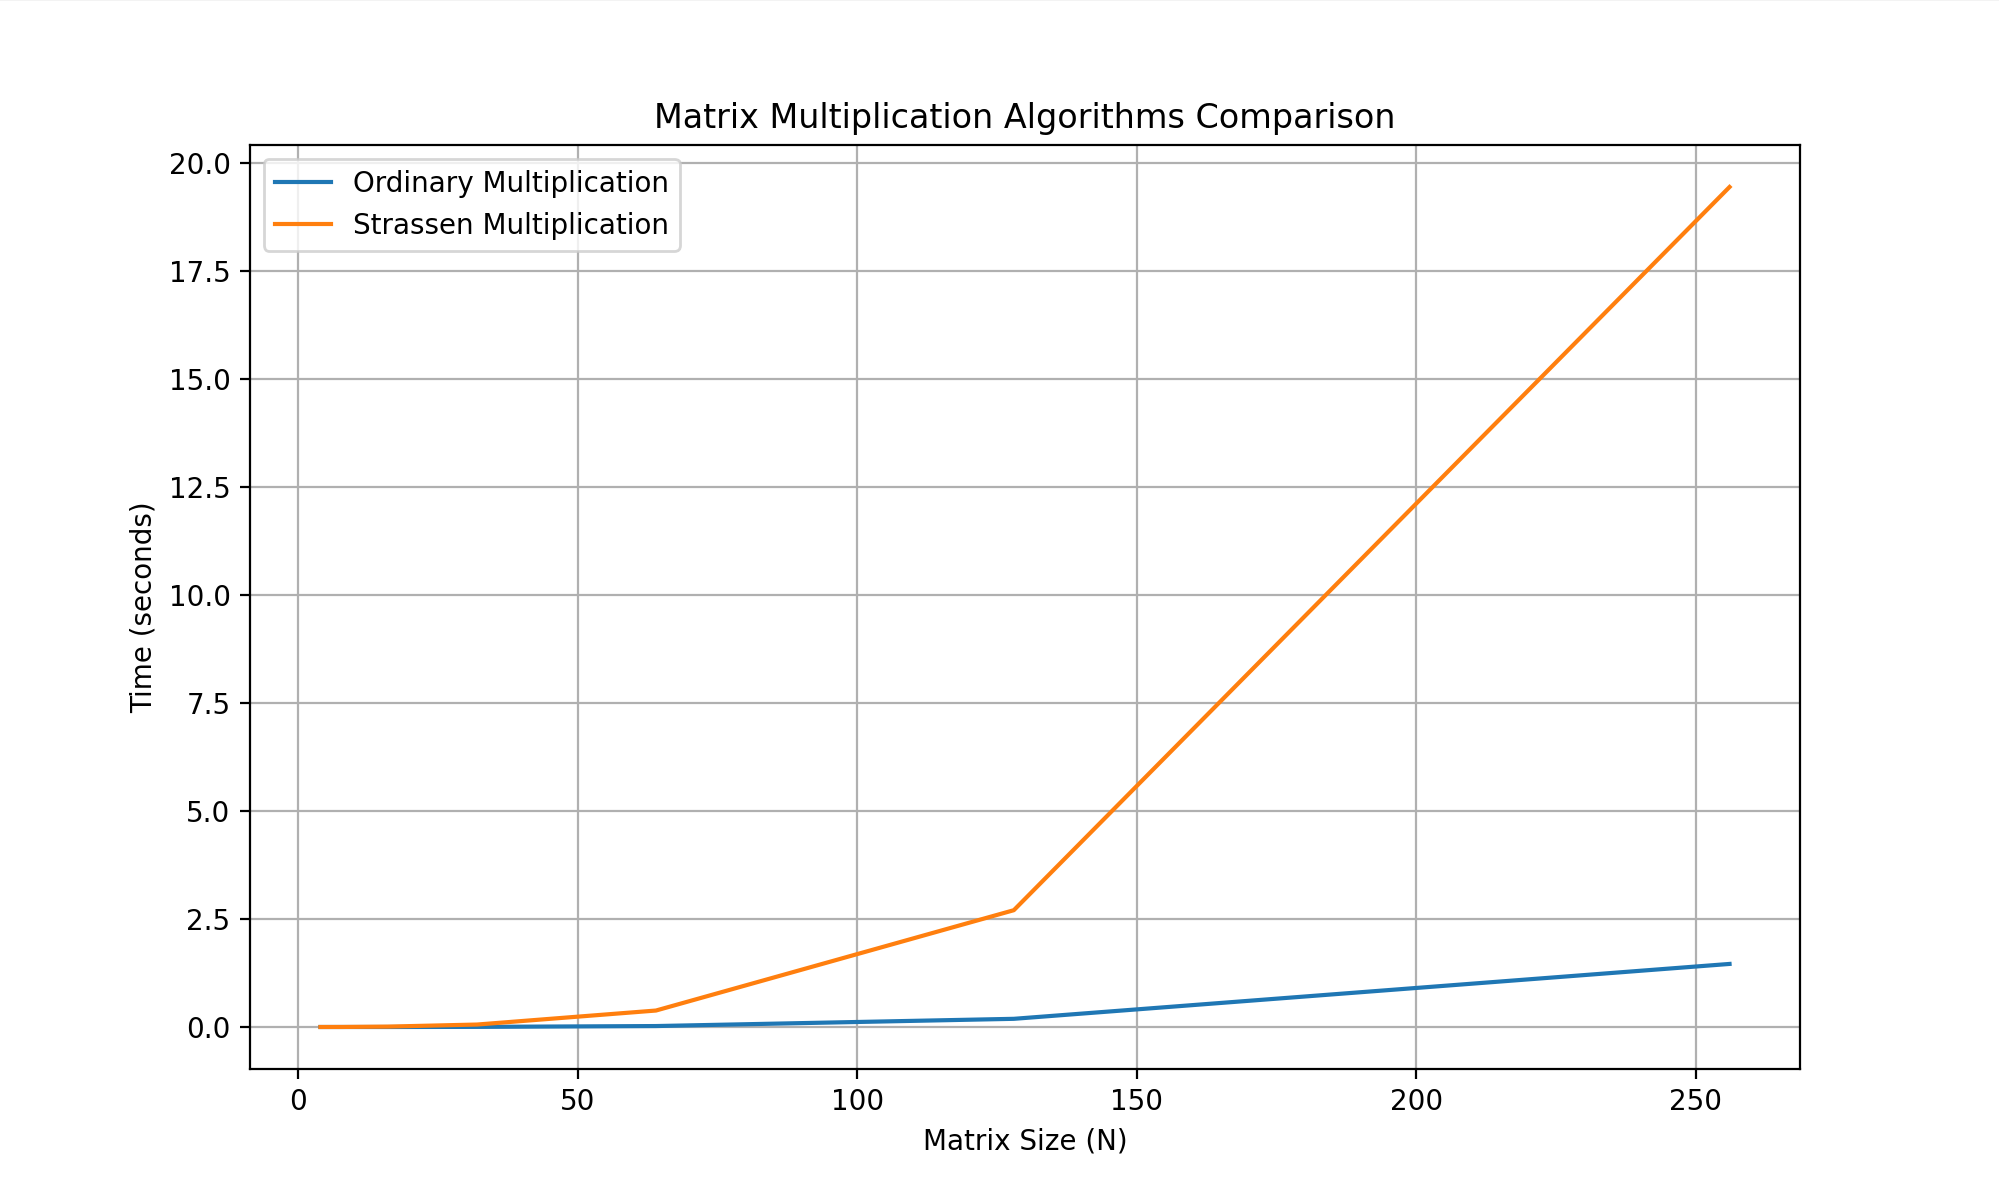
\includegraphics[width=0.8\textwidth]{Strassen_raw.png}
    \caption{Time cost of the ordinary algorithm and Strassen's algorithm}
\end{figure}
\medskip
\begin{figure}[H]
    \centering
    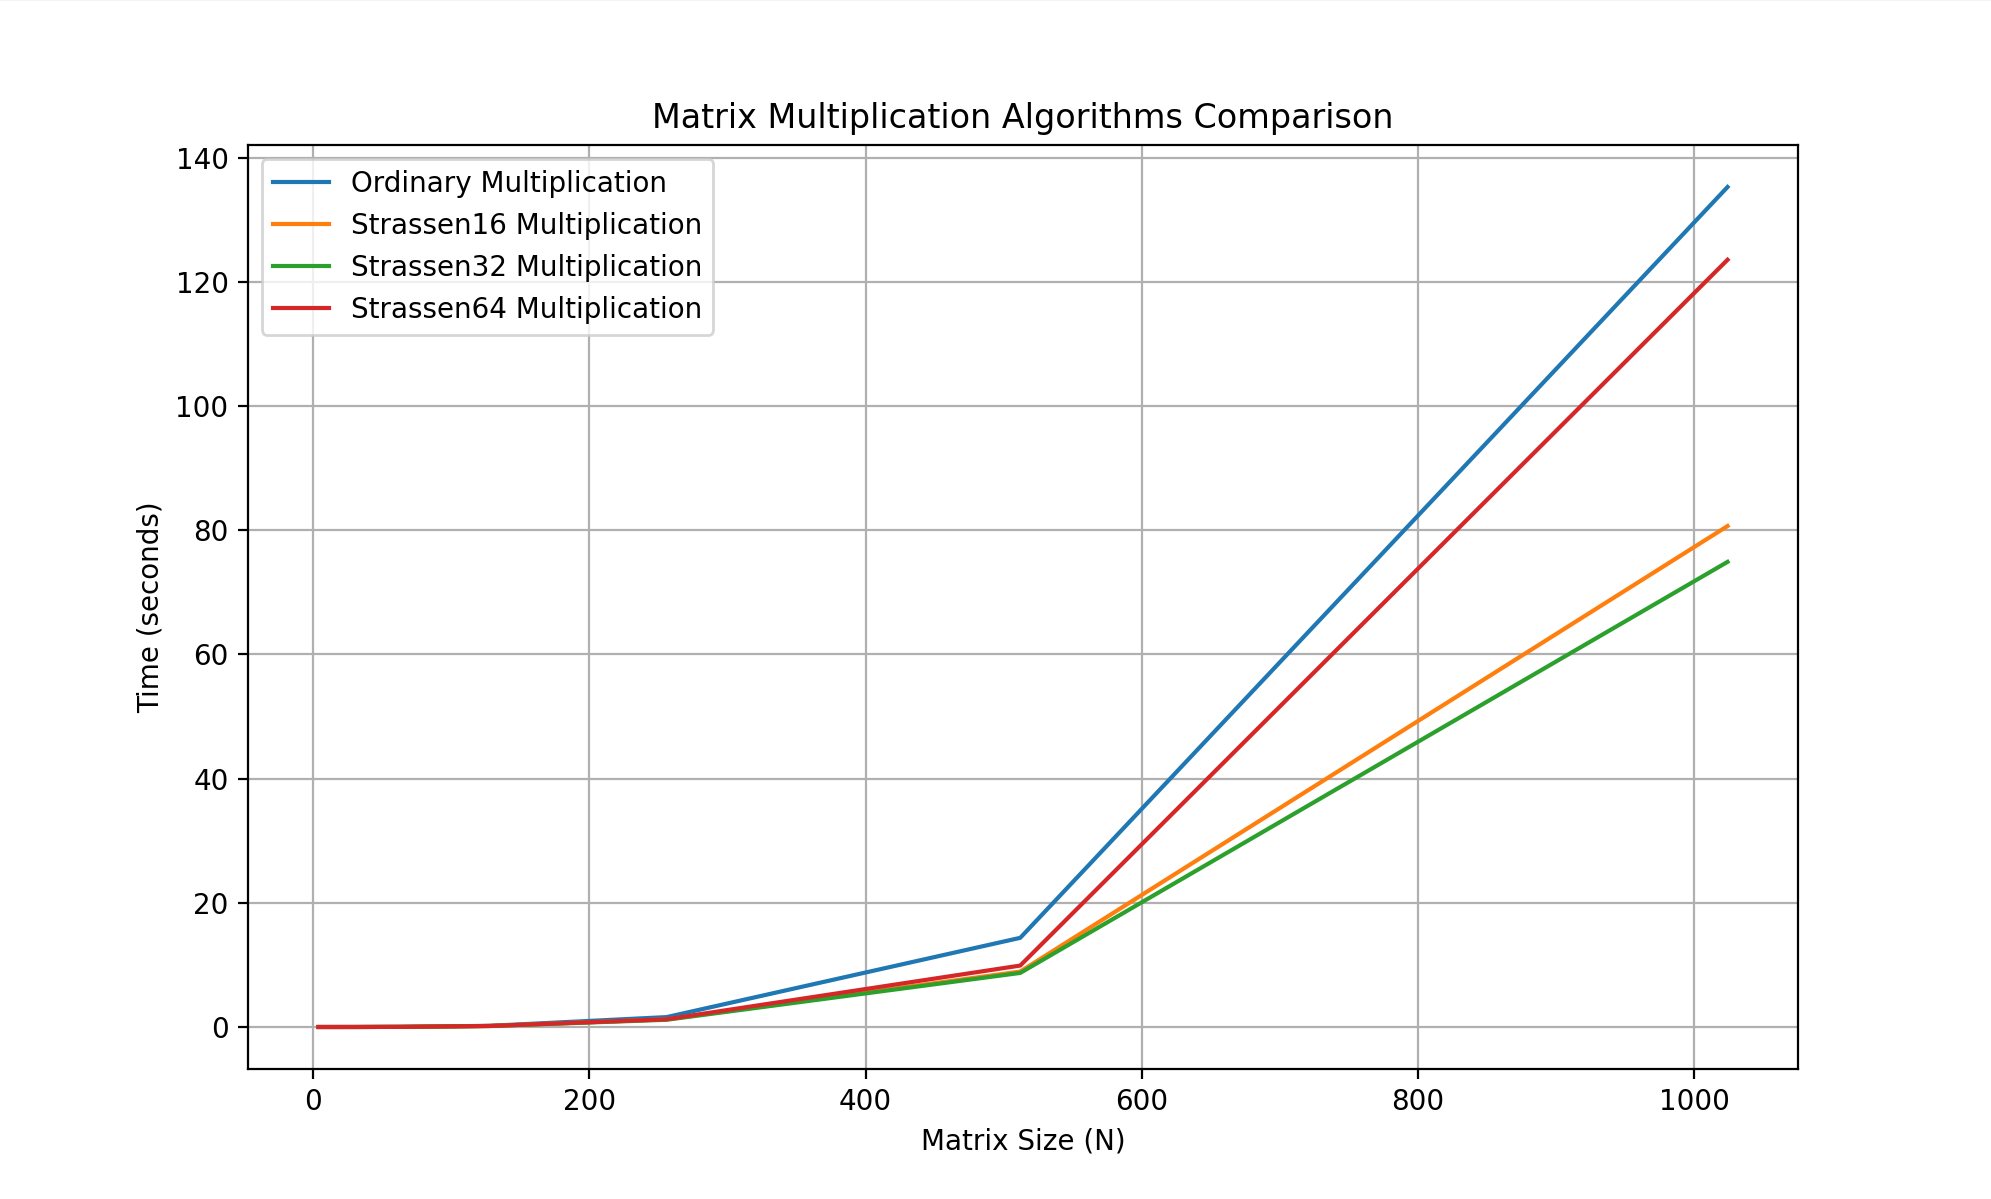
\includegraphics[width=0.8\textwidth]{Strassen_revised.png}
    \caption{Time cost of the ordinary algorithm and Strassen's algorithm with threshold}
\end{figure}
After improvement, the advantage of Strassen's algorithm is obvious when the matrix size is large, and the computation time is greatly reduced than the ordinary algorithm. This is consistent with the theoretical time complexity analysis.\\
Apart from that, we can see that $t = 32$ is good with the lowest cost among three thresholds. To further verify that the orders of magnitude of the two algorithms are correct, we take the cube root of the running time of the ordinary algorithm,
take $log7$ root of the running time of Strassen's algorithm, and draw a scatter plot. We use $\it{scikit-learn}$ package in Python to calculate both the linear regression models and compute their correlation coefficients to varify the linear relation.
The closer the absolute value of coefficient is to 1, the stronger the linear correlation is. Finally, we plot the regression lines. See code in timeana.py which is omitted here and results are shown in Table 2 and Figure 3 below.\\
\begin{table}[h!]
    \centering
    \caption{Regression and Correlation Results}
    \begin{tabular}{lcc}
    \hline
    & \textbf{Ordinary Method} & \textbf{Strassen32 Method} \\
    \hline
    Regression Equation & $y = 0.0050x - 0.0426$ & $y = 0.0045x - 0.0399$ \\
    Correlation Coefficient & 0.9995 & 0.9993 \\
    \hline
    \end{tabular}
\end{table}
\medskip
\begin{figure}[H]
    \centering
    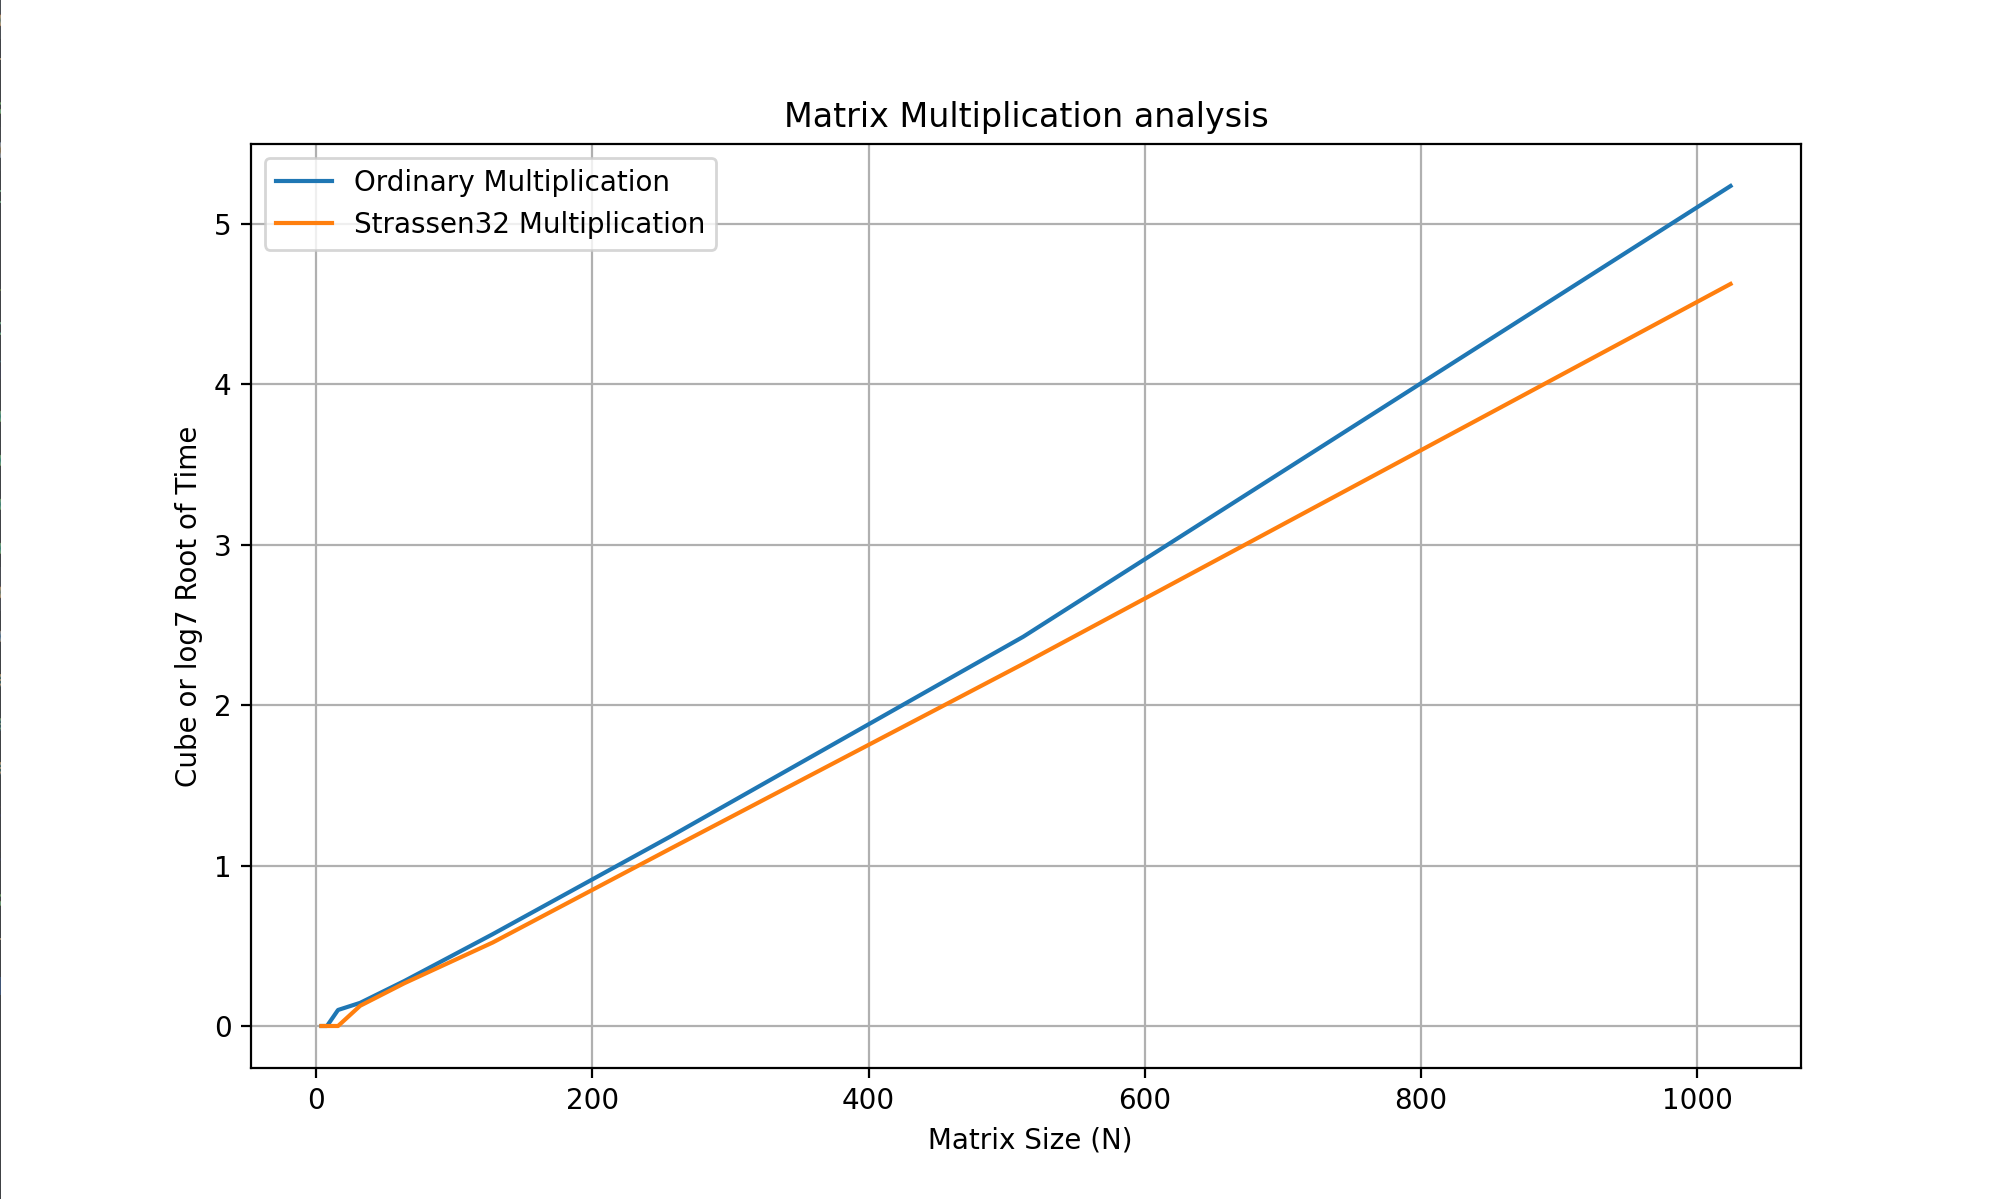
\includegraphics[width=0.8\textwidth]{complexity_analysis.png}
    \caption{Rooted time cost of the ordinary algorithm and Strassen's algorithm with threshold}
\end{figure}
From the table and the figure, we can see that the rooted time cost of the algorithm is much closed to a linear function of the matrix size, which is consistent with the theoretical time complexity analysis.\\
\textbf{Conclusion}:\\
The theoretical time complexity of the ordinary algorithm is $O(n^3)$, and the theoretical time complexity of Strassen's algorithm is $O(n^{log7})$. When the matrix size is large enough, Strassen's algorithm with thresholds is much faster than the ordinary algorithm.
However, when the matrix size is small, the ordinary algorithm is still useful.\\
\end{document}